\documentclass[]{article}
\usepackage{cite, graphicx}

\begin{document}

\title{Title}
\author{Author}
\date{\today}
\maketitle
\section{Dummy}

\subsection{Definition of the Data Model}
We describe the data model in an entity-relationship diagram. We create entities for all roles involved in the description of the system, and an entity for the Health Record. We abstract the attributes of the entities as much as possible. Note that the different read/write restrictions are not defined in this model:

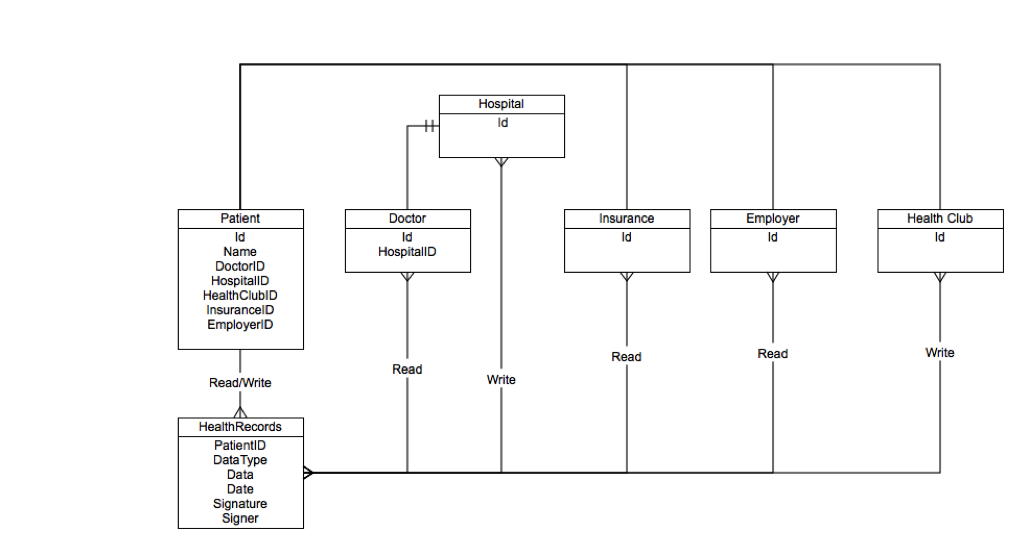
\includegraphics[width=350pt]{datamodel.png}

Note: 
\begin{itemize}
\item We include ‘type’ for health records. There are the following types of health records:
\begin{itemize}
\item General - e.g. Age, blood type, birth date, height, weight 
\item Medical - Information from medical service provider e.g. about surgery
\item Training - Information from Health club
\end{itemize}
We include a table (which is not displayed above) in the database that keeps track of  which signers are allowed to insert data in what time interval. This is needed to enforce access control for writing data (refer to the next chapter).


\subsection{Access Control Model}
We use an identity based proxy re-encryption scheme coupled with an identity based signature scheme to implement access control. Together these schemes allows us to implement the four access control requirements which call for fine-grained read + write permissions, and revocation. We describe the rationale in detail below.
\subsubsection{Fine-Grained Read Permission and Revocation}

Most cryptographic access control schemes such as ciphertext policy attribute based encryption (CP-ABE), proxy re-encryption and key policy attribute based encryption (KP-ABE) can be used to enforce fine-grained read permissions (i.e. decryption of ciphertext).

Unfortunately, both the CP-ABE and KP-ABE schemes do not efficiently support the additional (implicit) requirement to occasionally revoke read access to a patient's health records e.g. when Alice changes job, she needs to revoke the read access of her previous employer, Bob \& Co. We illustrate this with a simple CP-ABE scheme:
\begin{itemize}
\item Alice encrypts her medical health record granting access to attribute “Bob \& Co”. 
\item Bob \& Co's key contains this attribute.
\end{itemize}

We immediately see that it is not wise to revoke this attribute from Bob \& Co's key when a single employee leaves; The company would otherwise not be able to decrypt health records from its other employees. Instead, Alice needs to re-encrypt her health records with the attributes associated with her new employer, which could be a computationally costly operation if the data set is large. Hence CP-ABE, or mediated CP-ABE for that matter is not suitable; The same argument applies for KP-ABE.

Proxy re-encryption fills this gap nicely. In such a scheme, Alice can delegate a semi-trusted proxy to re-encrypt cipher text encrypted under her public key, to cipher text encrypted under Bob \& Co's public key. When Alice leaves Bob \& Co, she simply instructs the proxy to stop re-encrypting her health records to Bob \& Co. The proxy is ``semi-trusted'' in the sense that it has no access to the plain data and it will actually stop providing re-encryption keys to revoked entities.

Because proxy encryption allows the delegate full access to Alice's health records, we need as many key pairs as there are categories of her Health Record data to enforce finer grained granting of read access permissions (for example a HealthClub can only read Alice's training related data). The type-based proxy re-encryption scheme described in \cite{ibraimi2008type} would hence be ideal as it only requires a single key-pair to protect Alice's data which simplifies key management. Nevertheless, we choose to use Green's identity based proxy re-encryption scheme in \cite{green2007identity} primarily because there is a ready-to-use implementation in the Charm Crypto library \cite{charm13} which simplifies the implementation task. Green's scheme differs (effectively) from Ibraimi's scheme by having multiple keys for every identity and datatype combination. Furthermore, we only define only three types of data (General, Medical and Training) which results in a manageable set of keys for each Patient to store.

\subsubsection{Insert Permission}
The access control policy also calls for the granting of write permissions to select entities. Unfortunately, with the proxy re-encryption scheme described above, anyone can use the public key of an entity to encrypt data to the patient's database. The same is also true for CP-ABE and KP-ABE. As such we need an additional mechanism to control write access.

We hence choose to use an identity based signature scheme \cite{waters2005efficient} to enforce write permissions. An identity based system is ideal because there is no need to lookup public keys; moreover, the signing identity as the same identity used in the identity based proxy re-encryption. When an entity inserts data into a patient's record, that entity needs to sign that data, together with the insert date.

Example:
When Dr Frank wants to insert plaintext into Alice's health records, he stores the following into the HealthRecords table:\\
Ciphertext $=$ Enc(Plaintext, patientpublicKey)\\
Signature $=$ Sign(tuple, DrFranksigningKey), where tuple $=$ (Plaintext, Date of Signature)\\

The patient, and other entities who are allowed to read the patient's data, can check that the data is valid (i.e. inserted by the patient herself, or an authorised entity) by checking the AuthorisedInsert Table. This table is comprised of the Entity whom is authorised to write to a Patient's Health Record, the type of health record, and the date/time interval. The authenticity of this authorisation is validated by a Patient's signature. Because the time can be specified down to a second's precision, revocation of write permission is effectively instantaneous.

Our scheme compares favorably to the alternative method using a hash chain together with a signature scheme that was proposed by by Li et al in \cite{li2013scalable}. In Li's scheme, the patient delegates write permissions by providing the delegate with a hash (from the hash chain) corresponding to the authorised time interval. The patient simply stops issuing hashes at the time of revocation. We did not choose this method as it requires a trusted online presence to issue hashes, and because write access is tied to a time interval which might not be sufficiently granular.

\subsubsection{Assumptions}
\begin{itemize}
\item Some classical access control is provided to control access to the database e.g. passwords. Without this, anyone could modify data, hence invalidating signatures. This helps to protect the availability of files.
\item Although the proxy does not need to be trusted, still we need to make some assumptions on its correct operation:
\begin{itemize}
\item It generates re-encryption keys to the correct identity, as specified by the Patient
\item The proxy deletes re-encryption keys when instructed by the Patient. This helps to ensure proper revocation.
\item The proxy does not collaborate with users to decrypt a Patient's data.
\end{itemize}
\item A patient can have multiple doctors, hospitals, health clubs if she wants to.
\item The patient controls who has which access to her Health Record.
\end{itemize}

\subsection{Detailed Design}
\subsubsection{Introduction}
Our demonstrator is implemented in Python 3 and we use Green's proxy re-encryption scheme \cite{green2007identity} and Water's identity based signature scheme \cite{waters2005efficient} which are implemented by the Charm Crypto library \cite{charm13}. In this chapter we refer to Entities, which we define to include doctors, hospitals, insurance and health clubs but do not include the patients themselves.

Separately, we implement the Proxy, Patient and Entity class:
\begin{description}
\item[Proxy] The proxy class stores encrypted patient health records in a MySQL database. Patients and Entities interact with the proxy to read and write encrypted data. It also stores a dictionary of re-encryption keys which it uses to re-encrypt ciphertext from a Patient's key to an Entities’ key.
\item[Entity] The Entity class is used to instantiate Hospitals, Doctors, Insurance and Health Clubs. Entities can read and write to a (part of a) Patient's health records only if the Patient explicitly chooses to provide them access to a specific data type (General, Health, Training).
\item[Patient] The Patient class is used to instantiate different patients. Patients can read and write to their health records, and also delegate these permissions to entities.
\end{description}

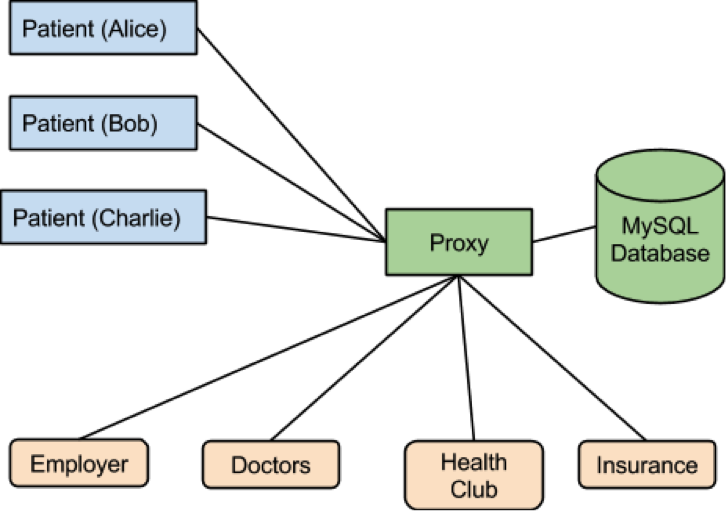
\includegraphics[width=200pt]{implementationmodel.png}

\subsubsection{Proxy}
The following functions are available in the Proxy Class. 

\begin{itemize}
\item init(): This function sets up the proxy re-encryption group with the security parameter 1024 and outputs the master secret key as an instance variable.
\item keygen(ID): On input an identity ID, a decryption key sk corresponding to that identity is returned.
\item addKey(ID1, ID2, rk): The re-encryption key (rk) which encrypts ciphertexts from the Delegator (ID1) to the Delegatee (ID2) is stored in a Python dictionary for future look-up.
\item listRk(): All available re-encryption keys are listed. Note that this just lists the delegator and delegatee and not the key itself.
\item reEncrypt(ID1, ID2, ciphertext): The ciphertext encrypted with the delegator's (ID1) key is re-encrypted with the delegatee's (ID2) key.
\end{itemize}
\subsubsection{Patient}
The patient class is used to instantiate patients. Patients have the ability to read and write to their own Health Records. The following functions are available for a patient:
\begin{itemize}
\item init(): This function instantiates a specific patient (ID), the connection to the proxy is set up and the signing key (signK) along with the master public key (masterPK) are given to the patient using this function.
\item store(recordType, msg): This function stores a message (msg) into the recordType part of the patient's own Health Record
\item read(recordType): This function reads the recordType part of the patient's own Health Record
\item verifySig(signerID, date, msg, signature): This function verifies the signature by signerID on a date on a specific message
\item addEntity(EntityID, HealthRecordType): This function grants read and write permissions to an Entity for a specific HealthRecordType for this patient's HealthRecord
\item revokeEntity(EntityID, HealthRecordType): This function revokes read and write permissions from an Entity to a specific HealthRecordType for this patient's HealthRecord
\item authoriseEntity(EntityID, HealthRecordType): Grants write access for an entity to a specific HealthRecordType for this patient's HealthRecord
\item revokeAuthorisedEntity(EntityID, HealthRecordType): Revokes write access for an entity to a specific HealthRecordType for this patient's HealthRecord
\item genRencryptionK(recordType, ID2): Grants read access to an entity (ID2) to a specific recordType for this patient's HealthRecord
\item removeRencryptionK(recordType, ID2, proxy): Revokes read access to an entity (ID2) to a specific recordType for this patient's HealthRecord
\item dec(recordType, ciphertext): sub-routine to decrypt a ciphertext stored in the recordType part of the patient's HealthRecord
\end{itemize}
\subsubsection{Entity}
The entity class is used to instantiate entities (Health Clubs, Doctors, Insurance and Hospitals). Entities have the ability to read and write to specific Patient's Health Records to which they have been granted access by the patient. The following functions are available for a Entity:
\begin{itemize}
\item init(): This function instantiates a specific entity (ID), the connection to the proxy is set up and a signing key (signK) along with the master public key (masterPK) are given to the entity using this function.
\item read(ID1, recordType): This function reads (and decrypts) data from a patient's (ID1) recordType which is a part of the HealthRecord
\item store(ID, recordType, msg): Store an (encrypted) message (msg) in a patient's (ID) recordType which is a part of the HealthRecord.
\item verifySig(signerID, date, msg, signature): This function verifies the signature by signerID on a date on a specific message
\end{itemize}

\subsection{Discussion and Conclusion}
There are many academic proposals to protect personal health records that utilise CP-ABE, KP-ABE and proxy re-encryption. Most of these schemes focus on the confidentiality of patient data by protecting read access. However, few schemes provide (or even mention) write access protection. Perhaps an underlying assumption of most authors is that write access protection is less important, or that classical access control is used. 

In this paper, we describe a practical and effective means to provide both read and write access control to a patient's health record which is a more realistic use case. This is achieved by combining identity based proxy re-encryption scheme together with an identity based signature scheme.

\bibliographystyle{plain}
\bibliography{Report_Part1}{}


\end{document}